% include the figures path relative to the master file
\graphicspath{ {./content/method/figures/} }

\section{Methodology}\label{sec:method}

Our approach is based on the original paper of Srinivasan~\textit{et al.} \cite{srinivasan2014fully} to which a feature extraction procedure (\gls{pca}) is added, as proposed by Venhuizen~\textit{et al.} \cite{venhuizen2015automated}.
Our general pipeline is presented on Fig.\,\ref{fig:fig3}.

First the image are preprocessed to remove the noise with the BM3D algorithm developed by Dabov et al.\,\cite{dabov2007image}; they are then flattened and cropped as described by Srinivisan~\textit{et al.} \cite{srinivasan2014fully} (see Fig.\,\ref{fig:fig4}).
\begin{figure}
\centering
\subfigure[Original]{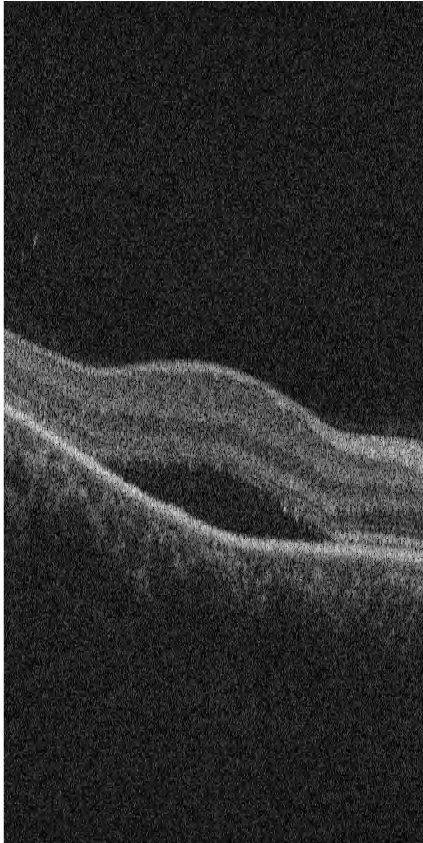
\includegraphics[width = 0.17\textwidth]{Original}}\
\subfigure[Flatten]{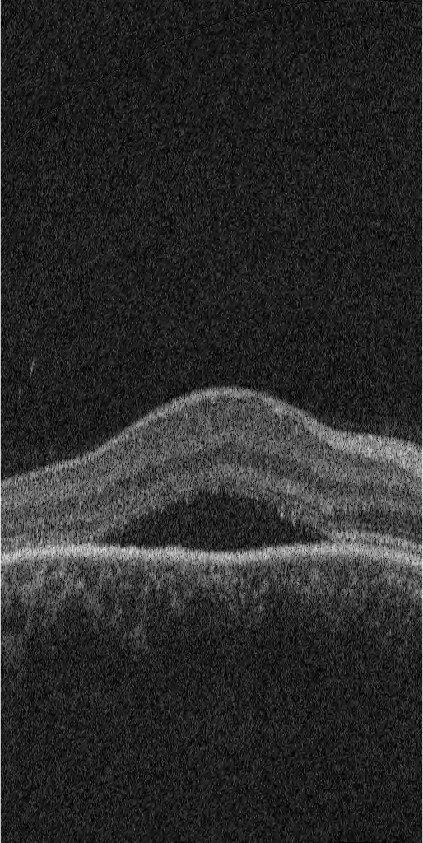
\includegraphics[width = 0.17\textwidth]{Flatten}}
\caption{Original and flatten image.}
\label{fig:fig4}
\end{figure}
On the cropped image, we extract \gls{hog} features \cite{dalal2005histograms} as well as \gls{lbp} features either in their standard version \cite{ojala2002multiresolution} or their rotation invariant version \cite{zhao2012rotation} with different neighborhoods.
Furthermore, to consider structures at multiple scale levels, both \gls{hog} and \gls{lbp} features vector are extracted at four levels of the multiscale Gaussian lowpass image pyramid.
For each feature, \gls{hog} or \gls{lbp} the histogram are concatenated into a single feature vector for each image.
Then the obtained histograms are either fed directly to a linear \gls{svm} classifier or reduced with \gls{pca}. 
We attempt to combine \gls{hog} and \gls{lbp} feature vectors or use them separately as explain in the next section.
